\chapter{Introduction}\label{chapter_introduction}
%% Describe the research area
\lettrine{S}{afety-critical embedded} system should be analyzed at the early stages of software development such as \emph{requirements specification}, \emph{software design} and \emph{software allocation} to ensure functional correctness in time, which is more effective and efficient than late analysis~\cite{bohm}.  Requirements specifications contain the functional and extra-functional requirements that are used in contractual terms and also are used in the subsequent development stages, e.g., design, implementation, verification and validation, etc., hence is vital to maintain good quality of requirements specifications~\cite{ieereqspecstandard}\cite{Siqueira2018ComparingReplication}. Likewise, software designs should realize the correct functionality of the system at hand before implementation and testing. The software designs are allocated to logical hardware components and units, which are usually constrainted in computation, I/O processing and power provision, thus should also be optimized to accommodate current and future embedded software functionality. In mode-based develpment, the different stages of system development are conceptualized using multiple levels of abstraction as in SysML, AUTOSAR, EAST-ADL, etc. architectural languages. 

Over the last decades \emph{formal methods} have attracted the interest of practitioners especially in the safety-critical area to ensure correct functionality at the various levels of system abstraction. Formal methods are mathematical techniques and tools which enable unambiguous specification and modeling, and rigurous analysis of systems, e.g., using theorem proving, model checking, satisfiability-moduo theories (SMT), etc \cite{o2017concise}.  Their applications have been stagnant mainly due to the difficulty of adapting to the mathematical jargon of the formal languages, lack of tools support, and scalability issues of the methods~\cite{Abrial2006FormalFuture}. As a result, it has become apparent in many cases that complete formal specification and modeling is usually impractical. Rather, formal methods should be
\begin{enumerate*}[label=(\roman*)]
	\item used like a ``swiss-army-knive'', that is simple, application oriented, mutiple techniques that are of orthogonal;
	\item ``lightweight'', that is with partial specification, modeling, and anlayiss on selected safety-critical functionality
\end{enumerate*}  \cite{lightweigh2001}.
In this thesis, we apply formal techniques in this manner to improve quality of requirements specifications and design models, thus we also consider or give focus to scalability and usability of the techniques in order to facilitate their applicability in industry.

Embedded systems requirements are usually expressed in natural language, thus sometimes are ambigous and incomprehensible due to its inherent ambiguity and extreme flexibility, though intuitive and expressive~\cite{ieereqspecstandard}. Template-based specification methods and controlled natural language are the two most commonly used approaches that bases on natural language to improve requirements specifications. The template-based specification methods, e.g., requirements boilerplates~\cite{Hull2011RequirementsEngineering}, etc.,  lack meta-model for extensibility and the template selection is usually cumbersome. Controlled natural languages, e.g., Attempto~\cite{attempto96}\cite{Fuchs2008AttemptoRepresentation}, etc., mimic the intuitiveness of natural language and have formal semantics, however, many lack domain specifity to embedded systems, hence are less effective. In this thesis, we propose the constrained natural language ReSA, which is domain specific to embedded systems and has formal semantics in Boolean logic and description logic. The Boolean representation enable shallow but scalable analysis of requirements, whereas the description logic representation enables deep (or rigorous) analysis but over limited requirements specifications.

%We apply the priciples to improve quality of requirements specifications and design models while giving special focus to scalability and usability of methods at the core of our approaches, in order to faciliate their applicability in industry.
% quality~\cite{ieereqspecstandard}\cite{Siqueira2018ComparingReplication}, e.g., unambiguous, consistent, comprehensible, etc. Similarly, embedded system designs must ensure the correct functionality and should conform to the specifications, before implementation. In this regard, 
%In this thesis, we propose rigurous analysis of embedded systems requirements and multi-rate design models using \textit{formal methods}. 



The dynamics of safety-critical embedded systems are usually modeled, simulated and anlalyzed before implementation. In this regard, Simulink is one of the most widely used development environment for multi-domain, multi-rate, discrete and continous safety-critical systems in industry. For this main reason, there is an increasing interest in formal analsis of Simulink models. Simulink Design Verifier, which is based on the Prover model-checker, is the de facto tool in the Simulink environment to formally verify Simulink design models. However, it has limited functionality, e.g., it supports only discrete models, has issues with scalability, and lacks verification of timed properties. In this thesis, we propose a less exhaustive, yet rigorous, scalable and robust analysis technique based on the statistical model checking \cite{bibid}, to detect functional and complex timing requirements, e.g., end-to-end timings, temporal order of actions, etc. In contrast to the exact model checking techniques, the statistical model checking technique uses adequate execution traces to properties of interest and scales better on the expense of less coverage.

In the presence of limited critical system resources such as processor, memory and power provision of embedded hardwares, safety-critical software with complex functionality, e.g., automotive functions, are distributed on multiple computing units to gain additional power of computation. Moreover, they can share execution platforms along non-critical software to improve efficiency following \textit{mixed-critical} design, which enables non-interference of software applications with different criticality. In this case, maximizing reliability of safety-critical software is crucial to meet high-level reliability goals to improve overall dependability of the system. Fault-tolerance is the most common technique to improve reliability but increases overhead of computation and consumes more power and energy. Therefore, it is crucial to make sure distributed safety-critical software systems are predictable, e.g., meet timing constraints and reliability goals, but also consumes less power to accommodate the ever increasing functionality of embedded software.

In the context of distributed computing, the timing and relibility analysis is not trivial while considering optimization of power cosumption due to the conflicting nature of the properties, e.g.,  to reduce the total power consumption of a distributed software, less processors (or computing units) are needed, however, to meet end-to-end timing requirements additional computing units may be required, which is also the case if the reliability of the system is need to be maximized such as by applying fault-tolerance in order to meet reliability goals. In this work, we propose an integrated approach to meeting the timing requirements and reliability goals while minimizing the total power consumption of the distributed system using exact and heuristic methods to efficiently allocate safety-critical and non-safety-critical software on network of computing units, with limited computation capability and power specifications.

Our research is evaluated on industrial automotive use cases and realistic benchmark. The requirements specification language ReSA and the Simulink models anlaysis are evalauted on the adjustable speed-limiter (ASL) and brake-by-wire (BBW) systems provided by Volvo Group Trucks Technology (VGTT). ASL is a speed limitation automotive function which controls the vehicle speed of Volvo trucks from speeding up and is useful in roads where speed-limitation signs are in place. The ASL use case consists of arund 300 functional and extra-functional requirements, architctural models in EAST-ADL, and Simulink models. The integrated software allocation is evaluated on the engine management system benchmark provided by Bosch~\cite{}, which consist of an AUTOSAR architecure with the timing specifications, activation mechanisms of schedulable objects employed to model the execution behavior of the system.


%In this thesis, we apply \textit{formal methods} to improve the qulaity of the requirements specifications and software designs which are mathematical techniques and tools for unambiguous specification and modeling, and rigurous analysis of systems, e.g., using theorem proving, model checking, satisfiability-moduo theories (SMT), etc~\cite{o2017concise} . Mainly due to the mathematical jargon, lack of engineer-friendly tools and scalability issues of the methods, their applications in industry are very limited \cite{lightweigh2001}\cite{Abrial2006FormalFuture}. To facilitate their applicability in industry, we apply the following principles:
%\begin{enumerate*}[label=(\roman*)]
%	\item ``swiss-army-knive'' technique, that is simple, application oriented, mutiple techniques that are orthogonal;
%	\item lightweight formal methods \cite{lightweigh2001}, that is with partial specification, modeling, and anlayiss on selected safety-critical functionality
%\end{enumerate*}.

%The exact and heuristic optimization techniques are used in many fields and in particular in the design space explaoration to find optimal and near optimal solutions, respectively. In the design of safety-critical embedded systems, power-consumption optimization is critical especially to battery-driven embedded systems, e.g., the electirical/electronic execution platform of vehicles. Moreover, powerful computing platforms are need to accommodate the growing complexity of embedded systems functionality. In modern electical/electronics architecture of vehicles, there are more than 200 automoitve functions, and execute millions lines of software programs. In contrast to other systems, it contains 7x Linux 3.1 kernel and 4x F-35 figher-jet lines of codes. As a result, efficient (or low-powered) design of embedded systems is important in order to accommodate the increasing demand of embedded software for power and energy provision from the execution platform. There a wide spread research especially on power and energy optimization at the hardwares level and at runtime using dynamic power and energy management software, e.g. using dynamic frequency and voltage scaling \cite{bibid}. There is little work during early design especially considering orthogonal effects such as timing and reliability on the total power consumtpion of a distributed software systems.

%In this thesis, we propose lightweight formal methods to improve the specifiation of embedded systems requirements, which are initially expresssed in constrained natural language, and to formally analyze large-scale Simulink models for functional and timing specifications. Furthermore, we propose an exact method  based on Integer Linear Programming to optimize the power-consumption of a distributed embedded software applications, and propose a hearistic approach basedon hybrid Particle Optimization (PSO) for large systems. The thesis contributions are summarized in the next subsection.

% State of the art + state of the practice
% - model-based development
%Componenent-based development and model-based development methods have been applied successfully to cope the difficulty of managing embedded systems development, e.g., via  reusuability, models, abstaction-levels (or view).  The development methods describe the various levels of system abstraction, e.g.,. architectural level (SysML, TAADL, AUTOSAR, EAST-ADL, etc.), behavioral level (e.g., Simulink, Modelica, etc.).  However, many of the languages and their frameworks lack support for rigorous analysis based on formal methods.  Likewise, to address the complexity, advanced computational architectures are introduced to accommodate the increasing demand of embedded software computations, e.g., in the automotive industry, 


%formal specification of embedded systems requirements in constrained natural language, ReSA, which is enriches the EAST-ADL requirement modeling with comprehensible and analyzable  with formal specification of requirements that is analyzable using SMT solvers, furthermore, the thesis proposes a method to formally analyze industrial Simulink models using statistical model-checking. Furthermore, to verify functional and timing properties. Statistical model-checking is a formal technque which uses traces of system executions to check if properties hold in the system model. Unlike with exact model-checking, which suffers from state-explosition, statistical model-checking is scales well, albiet not exact.
%In 2015, the embedded hardwares market share was 93\% and is projected to grow by CAGR 6.36\% until 2021 \cite{bibid}, of which the automotive share accounts for 25\%. The latter is mainly driven by the advancement in driver-assistance, active-safey features, and emergent (hybrid) electric and self-driving vehicles.  As compared to 2000, the number of software applications running on electrical/electronic vehicle architecture have increased by x, and likewise, the number of lines of code increased by x.
% - existing solution:
% - what is lacking


% highlight the problems that you want to address in the thesis
% - requirements specifications: ambiguous, incomprehensible, inconsistencies
% - resource efficiency
% - software design errors, e.g.,timing errors
%Thus, in this thesis, we propose methods to assist rigorous analysis of specifications and systems models at different levels of systems abstraction following the EAST-ADL and AUTOSAR architectures. Moreover, we propose a distributed architecture that entertains the timing and reliability requirements of software applications via efficient deployment on heterogeneous computation nodes (with respect toprocessor speed, power consumption). In summary, the contributions of thesis are described as follows:¨
%In this thesis, we propose lightweight formal techniquesd to improve requirement of embedded systems requirements, to analyze large-scale Simulink models, and a power-efficient allocation of mixed-critical software allocation on network of computation units. The thesis contributions are summarized in the following subsection.

\section{Research Contributions Overview}
In this subsection, we give overview of the thesis contributions, and later in Section x, the contributions are further discussed in detail.
\begin{itemize}
\item \textbf{Formal Analysis of natural language requirements: } Most software and system requirements of embedded systems are specified in natural language, in fact it has become the de facto standard in industry, which is mainly because it is intuitive as opposed to computer languages, but also is expressive and flexible that many software engineers and other stakeholders find it easy to use. However, it is inherently ambiguous and therefore could lead to ambiguous and incomprehensible specifications. 
As opposed to the use of templates \cite{Hull2011RequirementsEngineering}, specification patter systems\cite{Gruhn2006PatternsSpecifications,Konrad2005Real-timePatterns} , we propose a fairly expressive, flexible yet structured and domain domain-specific language, called \textit{ReSA} [ref] that utilizes the EAST-ADL architectural language to improve its effectiveness by reducing syntactic and semantic ambiguities of specifications. The language has translation in Boolean and description logic to support rigorous analysis using existing formal method tools, e.g., SMT solving, reasoners (inference engines) to detect, e.g., logical inconsistencies. Moreover, by translating interesting specifications to TCTL and WMTL properties, the language can be used to abstract syntactic complexity there by simplifying properties specification, e.g., for use in the model checking of Simulink model, after translation to formal model as briefly discussedin the next contribution.
\item \textbf{Scalable analysis of Simulink models: }
Many safety-critical embedded systems are developed in Simulink \cite{JamesB.Dabney2003MasteringSimulink}, which is the de facto modeling language employed in industry.To provide assurance that Simulink models fulfill given functional and timing requirements, we propose a pattern-based, execution-order preserving automatic transformation of atomic and composite Simulink blocks into stochastic timed automata that can be formally analyzed using UPPAAL Statistical Model Checker \cite{Bulychev2012UPPAAL-SMC:Automata}. Our method is scalable, and has been validated on industrial use cases \cite{Filipovikj2016SimulinkSystems}. The statistical model checker analyzes a state-transition system by conducting statistical analysis on the collected traces of the system executions, effectively mitigating the state-space explosion of (exact) model checking \cite{Legay2010StatisticalOverview}. 

\item \textbf{Deployment optimization of distributed software applications: }
At the system design level, the requirements specifications are realized by a system architecture of software and hardware parts that are constructed by functional components (or modules) that abstract the functionality of the system. In the platform-based development approach \cite{Sangiovanni-Vincentelli2004BenefitsDesign}, the system design should take into account consumption of critical hardware resources, such as power consumption, for two main reasons: optimizing power consumption is beneficial in order i) to accommodate more applications as well as to support power-intensive applications, and ii) to increase battery-life by lowering the amount of heat released by electronic components in the system. In this thesis, we propose an exact software allocation approach, as well as a heuristic one, for multirate systems that need to meet both timing and reliability.
\item \textbf{Validation on industrial use cases: } 
Our contributions such as its the ReSA language as well as the proposed formal analysis of Simulink model is validated on industrial use cases, which are provided
\end{itemize}
\begin{figure}
	\centering
	\ifpdf
	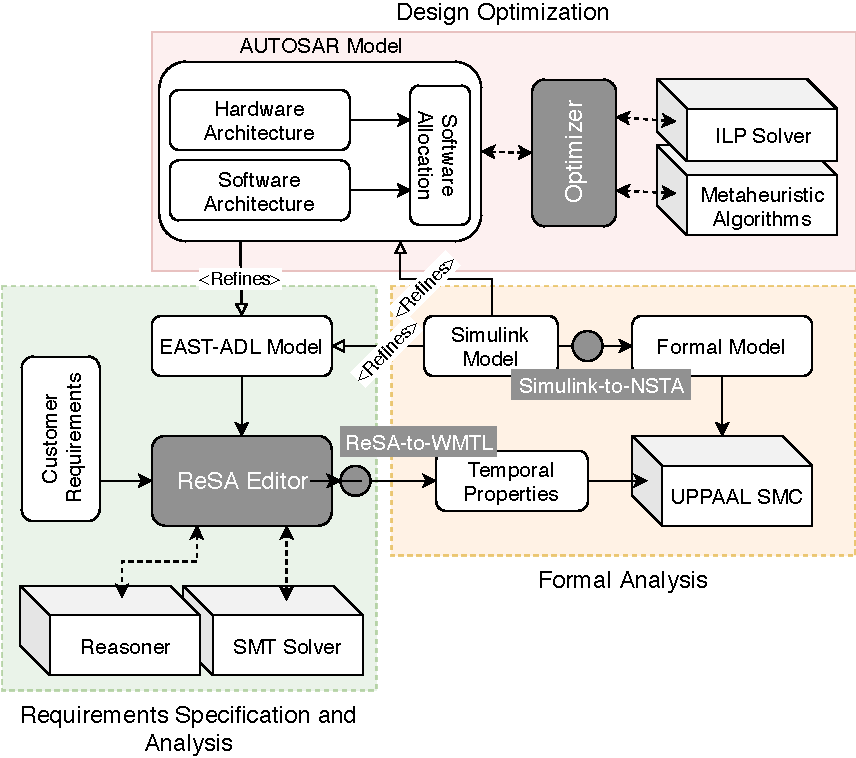
\includegraphics[width=\linewidth]{images/softdevflow}
	\else
	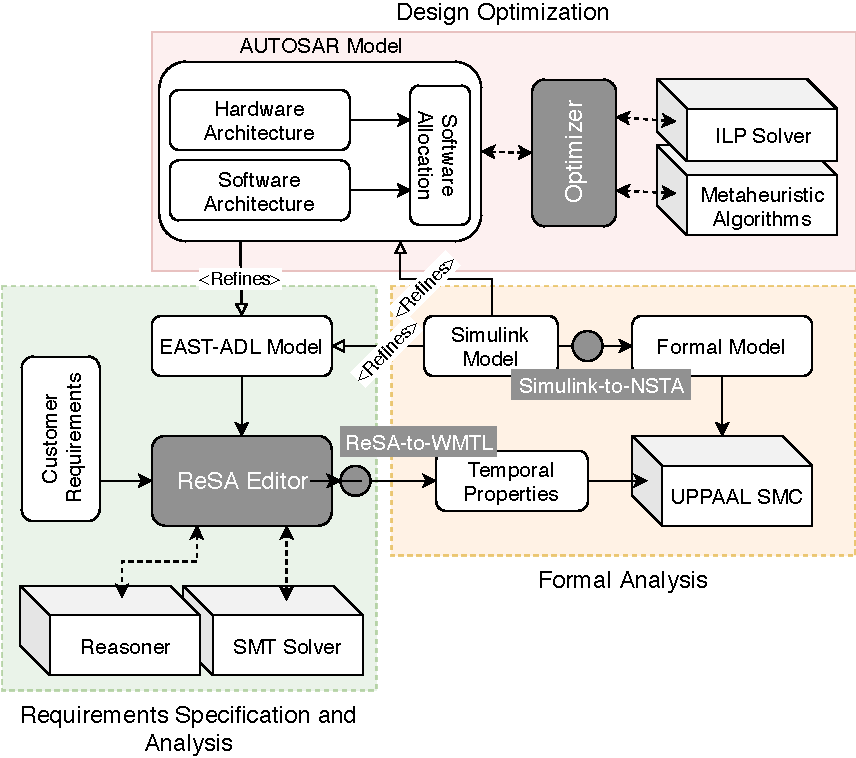
\includegraphics[width=1.0\linewidth]{images/softdevflow.eps}
	\fi
	\caption{Thesis Contributions Workflow.} 
\end{figure}

The rest of the thesis proposal is organized as follows. Section \ref{section:goals} introduces the research goals and the scientific contributions to address the research goals. Section \ref{section:methods} presents the research methods applied to conduct the research especially in the context of academic-industry collaboration. Section \ref{section:outline} shows the proposed outline of the thesis, followed by the presentation of the research progress in Section \ref{section:progress}, including the time plan until the doctoral defense. Section \ref{section:thirdcycle} presents the third-cycle outcomes, adapted from the individual study plan (ISP). Finally, Section \ref{section:related} discusses the related work before concluding the proposal in Section \ref{section:conclusions}.

\section{Thesis Outline Overview}
The thesis is divided into two parts. The first part is a summary of our research. It is organized as follows: in Chapter 2, we give the background information on description logic, Boolean satisfiability problem, Simulink, stochastic timed automata, and meta-heauristic optimization. In Chapter 3, we explain the research problem and outline the research goals. The thesis contributions are discussed in Chapter 4, followed by the related work in Chapter 5. In Chapter 3, we describe the research method applied to conduct the research. Finally, in Chapter 7, we conclude the thesis and outline possible directions for future work.

The second part is a collection of papers included in thethesis, and briefly described listed as follows: